

%A continuación, se presentarán los casos de uso a los que se pretende atender con el simulador desarrollado.


\section{Courseware}
\label{xray:courseware}

El módulo \ac{Courseware} es el responsable de proporcionar las capacidades de entrenamiento al simulador, al hacerse cargo de la gestión de los módulos de posicionamiento y de simulación de rayos X. Proporciona una \ac{IU} que permite la interacción con los distintos módulos y la funcionalidad específicamente diseñada para el entrenamiento.
\begin{figure}
    \centering
    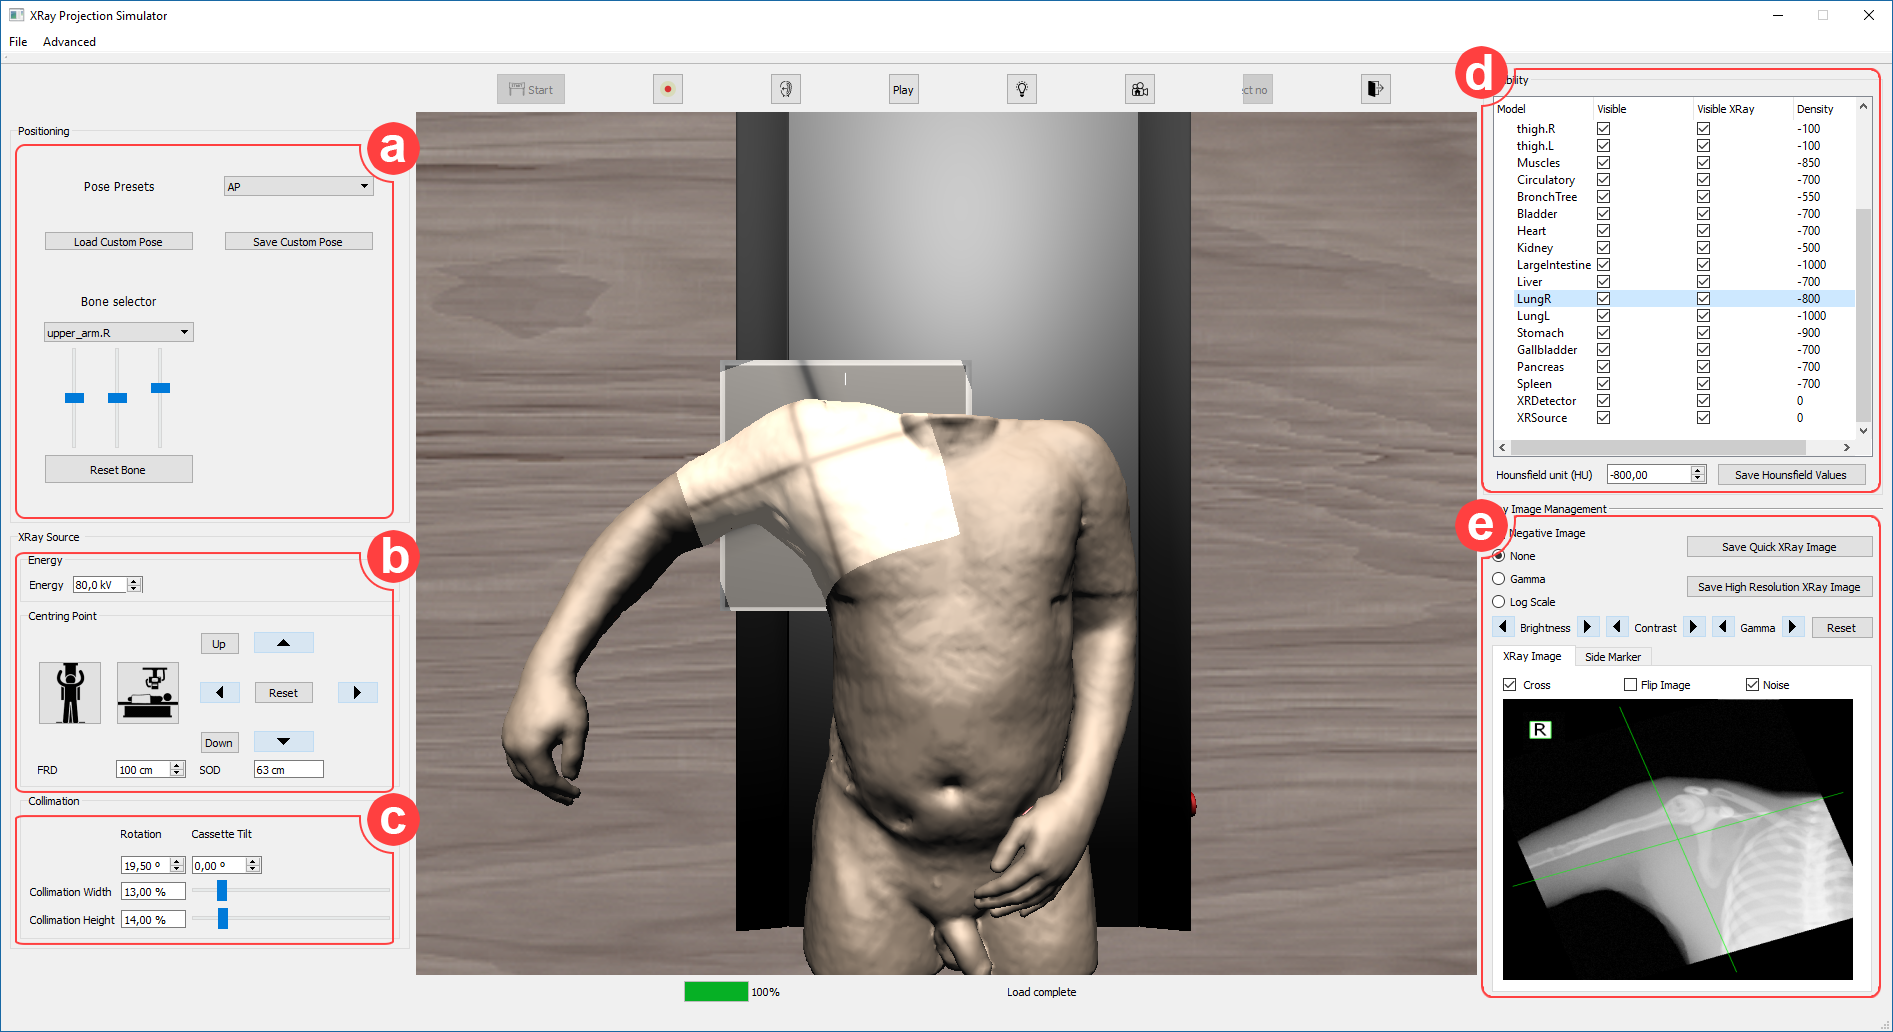
\includegraphics[width=\linewidth]{IMG/uiteacher.png}
    \caption{\acs{IU} del simulador de radiología diagnóstica : (a) Posicionamiento del paciente virtual;  (b) Configuración de la máquina de rayos X; (c) Configuración de la colimación; (d) Configuración de la visibilidad y propiedades físicas de los distintos tejidos; (e) Posicionamiento de los marcadores de referencia y ventana donde se observa la radiografía.}
    \label{fig:uiusecase}
\end{figure}

En la figura \ref{fig:uiusecase} se muestra la apariencia de la \ac{IU} y las principales funcionalidades del simulador. En la esquina superior izquierda se localizan los botones para el posicionamiento del paciente virtual. Más abajo, se encuentran los botones que dan valor a los parámetros que configuran la máquina de rayos X. En la esquina inferior izquierda se localiza la configuración de la colimación. En la esquina superior derecha, se encuentra la lista de anatomía presente, donde se podrá modificar su visibilidad o sus propiedades físicas.  Finalmente, en la esquina inferior derecha, se muestra la imagen de rayos X en tiempo real. En esta misma subdivisión, en otra pestaña, se encuentra la herramienta para colocar el marcador de referencia.

A continuación, se describen las funcionalidades más importantes de este módulo. Primero se explicará como se ha caracterizado el procedimiento (la descripción del completa del procedimiento se puede consultar en la sección \ref{art:xraysim}) y por último las funcionalidades de herramienta de clase y aprendizaje autónomo.




\subsection{Posicionamiento del paciente virtual}
\label{xray:posing}

En el diagnóstico por imagen, la posición del paciente es esencial para poder obtener la mejor imagen médica, evitando repeticiones y exposiciones adicionales a los rayos X. La comodidad y la seguridad del paciente es fundamental y los profesionales de radiología tienen que estar seguros de como colocar al paciente. Como se describe en \cite{carver2012medical,manualpractico}, el usuario debe elegir la posición del paciente (de pie o tumbado) ya que este aspecto es relevante médicamente y es importante en el currículum de los estudiantes.

En este simulador, gracias al algoritmo propuesto en esta tesis, %el usuario es capaz de modificar la postura del modelo anatómico cargado con el objetivo de aprender a conseguir una pose correcta. 
los usuarios pueden interaccionar con el simulador a través %de la \ac{IU}
de tres formas. Se pueden elegir una pose entre una lista posiciones predefinidas anteriormente. Es posible, también, seleccionar y mover una a una las articulaciones de las que disponga el paciente virtual. Por último, se puede estimar una posición utilizando \ac{MoCap} o con dispositivos como Microsoft Kinect (ver sec. \ref{posing:Poses}). 
%
En la figura \ref{fig:pose}, el brazo ha sido posicionado con el objetivo de conseguir una proyección lateral de húmero. Cualquier posición seleccionada puede ser almacenada para futuros usos.



% \begin{figure}
%      \centering
% 		\subfigure[]{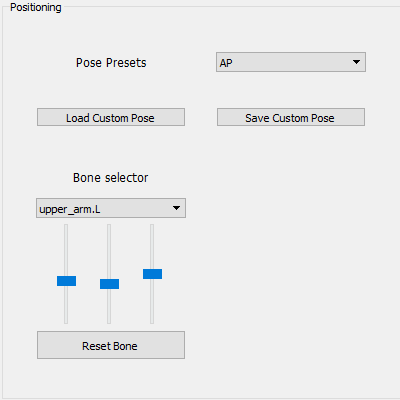
\includegraphics[width=0.45\linewidth]{IMG/PoseUI.png} A user defines the left arm position via the . \label{subfig:position} }
% 		\subfigure[]{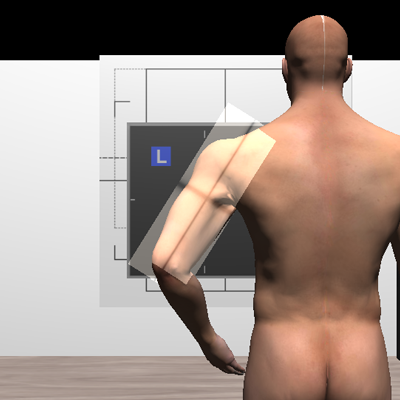
\includegraphics[width=0.45\linewidth]{IMG/PoseArm.png} Corresponding 3D visualisation where the virtual patient's left arm has been moved accordingly.\label{subfig:US-B}}
		
% 		\caption{\label{fig:pose} {An example of virtual patient positioning.}}    
% \end{figure}


\begin{figure}[ht]
    \begin{subfigure}[b]{0.45\linewidth}
        \centering
        {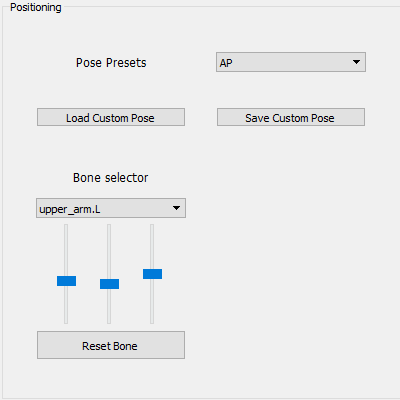
\includegraphics[width=\linewidth]{IMG/PoseUI.png}}
        \caption{El usuario utiliza los actuadores para definir la posición del brazo izquierdo. \label{subfig:position}}
    \end{subfigure}
    \null\hfill
     \begin{subfigure}[b]{0.45\linewidth}
        \centering
        {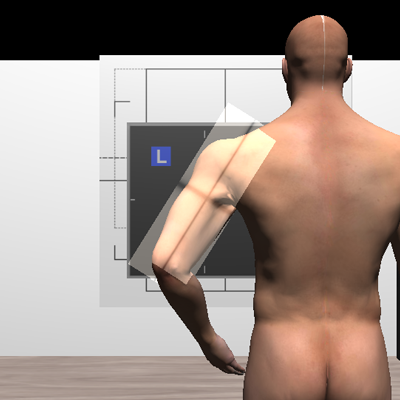
\includegraphics[width=\linewidth]{IMG/PoseArm.png}}
        \caption{Escena 3D resultante del paciente virtual con el cambio de posición del brazo izquierdo.\label{subfig:US-B}}
    \end{subfigure}
    \caption{\label{fig:pose} Ejemplo del posicionamiento del paciente virtual en el simulador.}
   \end{figure}



\subsection{Configuración de la máquina de rayos X}
\label{xray:setupxray}

Los factores de exposición son un aspecto fundamental en el diagnóstico por imagen ya que afecta tanto a la seguridad del paciente como a la calidad de la imagen radiológica. Una configuración inapropiada del emisor puede producir un mal contraste en la imagen, siendo el objetivo final prevenir repeticiones innecesarias.

La simulación de rayos X está definida por varios parámetros: el emisor y el detector de rayos X (o chasis), y los modelos anatómicos que serán virtualmente irradiados. 
\begin{itemize}
    \item Emisor: definido por su posición, forma y espectro de emisión. Permite simular la forma que tendría la fuente de fotones de una máquina de rayos X (un punto, una línea, un cubo o un conjunto de puntos). Además, se puede configurar su espectro de emisión a través de una lista discreta de protones que tienen la misma o diferentes energías.
    \item Detector: es definido por un plano con su posición, tamaño, resolución y orientación. El plano se traduce en el número de \emph{píxeles} que tendrá la imagen final (ratio tamaño-resolución), y por consecuencia, definir el número de rayos que simulará la librería. Normalmente, este plano se encuentra perpendicular a la dirección de los rayos, pero no es estrictamente necesario.
    \item Modelos anatómicos: se utiliza su representación superficial acompañado de sus propiedades físicas. Estas propiedades se pueden definir a través de su composición química (porcentaje de átomos de determinado elemento químico) o por su radio-densidad definida por la escala \emph{Hounsfield}. Esta escala es más habitual en entornos médicos. La conversión entre las dos definiciones es posible gracias a \cite{Schneider2000}. Las propiedades físicas de las mallas superficiales son usadas para calcular los coeficientes que se usarán en la ley de atenuación para cada espectro del haz incidente. La correspondencia entre ellos se puede consultar en la base de datos \emph{XCOM} \cite{XCOM}.
\end{itemize}

Además de los parámetros que se corresponden directamente con valores que se pueden configurar en la librería \emph{gVirtualXRay}, se han desarrollado funcionalidades que permiten simular los aspectos más importantes y significativos para la correcta caracterización del procedimiento de radiología diagnóstica. 

%Centraje
El centraje (en inglés centring) y el posicionamiento del paciente son aspectos críticos del procedimiento para colocar correctamente la anatomía objetivo en el centro de la proyección. Esto es fundamental para reducir la cantidad de radiación que recibe el paciente. El radiólogo tiene que asegurarse que la zona anatómica objetivo está en el centro de la proyección y del panel del detector. Además, el usuario debe seleccionar la distancia que hay entre el emisor de rayos X y el detector (conocida como distancia foco-película).

%colimacion
La colimación es otro paso fundamental del procedimiento. Es la técnica de limitar la proyección del haz saliente del emisor con unas placas de plomo. El plomo es un material muy eficaz que permite atenuar la radiación de los rayos X. Esta técnica es importante para limitar el área irradiado de la anatomía del paciente y, por tanto,  disminuir la radiación que recibe el paciente. También reduce la dispersión de la radiación y mejora la calidad de la imagen.

Todos estos parámetros han sido introducidos en el simulador como parte importante del procedimiento, donde los estudiantes o profesores pueden practicar o enseñar estos conceptos. A través de la interfaz 3D los usuarios pueden centrar con el ratón la luz proyectada desde el emisor y configurar la colimación (ver fig. \ref{fig:collimation}) o pueden usar los botones de la interfaz para conseguir una buena colocación de la proyección (ver fig. \ref{fig:setup}).

\begin{figure}[tb]
\centering
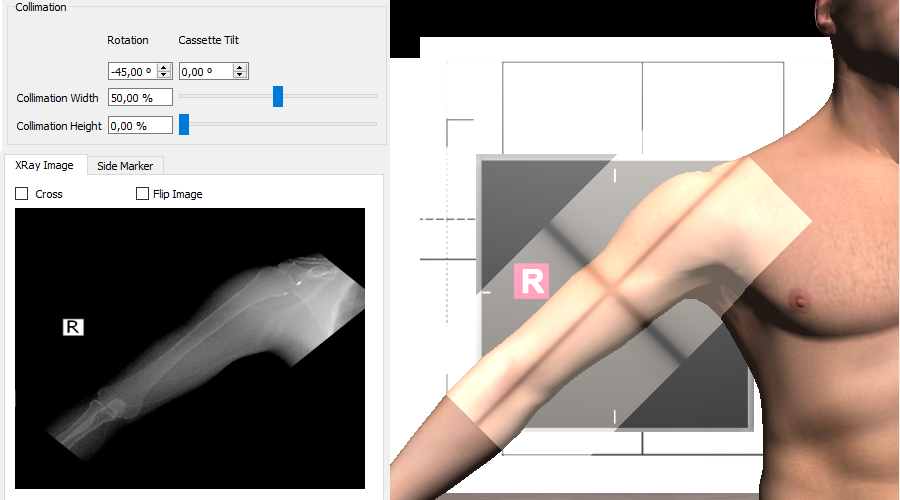
\includegraphics[width=0.9\linewidth]{IMG/collimation.png}
\caption{\label{fig:collimation} Ejemplo de colimación para conseguir una imagen limitada al húmero. Se ha reducido la distancia foco-película y la proyección ha sido rotada  45º. }
\end{figure}

Otro aspecto fundamental del procedimiento es la configuración energética de la máquina de rayos X. Con el objetivo de evitar errores y repeticiones, los estudiantes deben entender como el emisor de rayos X produce la radiación y que parámetros afectan a la calidad de la imagen. El emisor se compone de un cátodo que produce electrones y un ánodo donde los electrones chocarán. Si los electrones llegan con la suficiente energía, se generarán rayos X en una determinada dirección. Un operador puede controlar el tiempo de exposición en fracciones de segundo y los parámetros energéticos (tensión eléctrica aplicado al emisor en \ac{kV} y una intensidad en \ac{mAs}). El voltaje controla la energía de los fotones producidos por el emisor. Por otra parte, la corriente controla la cantidad de fotones producidos en un determinado tiempo (segundos). 
Para el radiodiagnóstico, el ánodo suele estar fabricado con tungsteno. Los voltajes más comúnmente usados se encuentran entre 55-125~\ac{kV}. El correspondiente espectro resultante puede ser simulado por la herramienta \ac{TASMIP}~\cite{Boone1997}. Por cada voltaje entre ese rango, produce un espectro de fotones, medidos en \ac{keV}. El usuario puede seleccionar el voltaje \ac{kV} objetivo, y \emph{gVirtualXRay} generará el espectro correspondiente.

La variación del voltaje seleccionado afecta a las radiografías, ya que la radiación de los rayos X es absorbida de forma diferente entre los tejidos blandos y densos. El nivel de absorción varía de forma no lineal según la energía del fotón. 
Por una parte, si el usuario configura un valor de voltaje demasiado bajo, la imagen resultante estará desenfocada y blanquecina. Por el contrario, si el valor del voltaje es demasiado alto, la imagen quedará sobre-expuesta resultando en una imagen muy oscura.

En la figura \ref{fig:setup}, se puede observar la diferencia entre dos configuraciones del emisor diferentes. El usuario puede jugar con los parámetros que le ayudarán a entender como los cambios en el voltaje afectan a la imagen de manera inmediata. Hay que destacar, que el comportamiento determinista de la librería \emph{gVirtualXRay} impide la simulación de la corriente (\acs{mAs}). Sin embargo, un valor bajo de \ac{mAs} puede imitarse añadiendo un ruido de \emph{Poisson} a la radiografía resultante.


% \begin{figure}[tb]
% \centering
% \includegraphics[width=0.5\linewidth]{IMG/setup.png}
% \caption{\label{fig:setup} Ejemplos distintos de configuración del emisor. Arriba podemos observar sobre exposición y una imagen más oscura. Por otro lado, abajo hay poca exposición que resulta en una imagen borrosa y blanquecina. }
% \end{figure}

\begin{figure}[ht]
    \begin{subfigure}[b]{0.9\linewidth}
        \centering
        {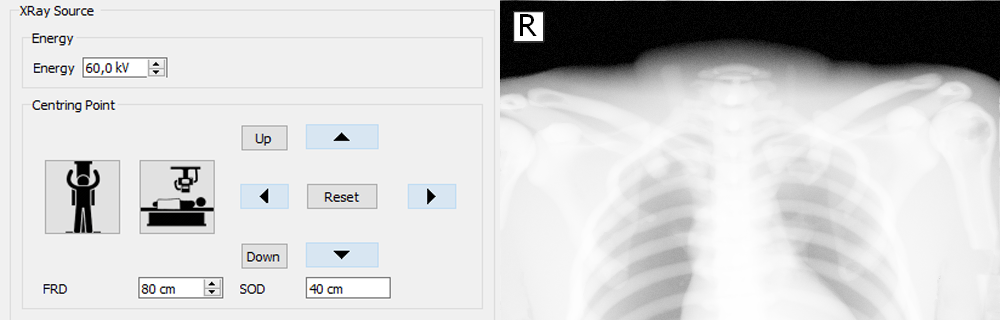
\includegraphics[width=\linewidth]{IMG/60kvp.png}}
        \caption{Radiografía obtenida con un valor de 60~\acs{kVp}.  La energía incidente es demasiado baja para penetrar en los tejidos, lo que resulta en una imagen blanquecina.\label{fig:60kvp}}
    \end{subfigure}
    
     \begin{subfigure}[b]{0.9\linewidth}
        \centering
        {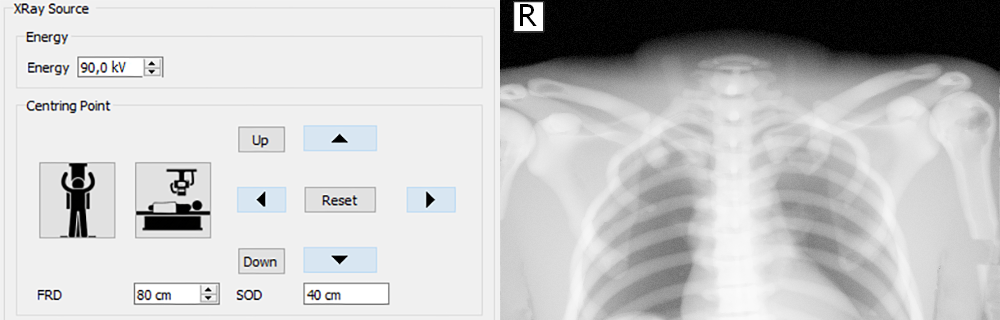
\includegraphics[width=\linewidth]{IMG/90kvp.png}}
        \caption{ Radiografía resultante de configurar 90~\acs{kVp}. En esta ocasión, el contraste entre tejidos ha mejorado.\label{fig:90kvp}}
    \end{subfigure}
    \caption{Efecto en una radiografía de pecho de la configuración del voltaje del emisor de rayos X. \label{fig:setup}}
   \end{figure}
   
   %\todo{Me he dado cuenta que la imagen no coincide con el texto, a la espera de Franck para aclararlo. Te lo había puesto!!!!! Me lo había puesto yo.}


%\subsection{Centro de proyección y colimación}
  
\subsection{Marcadores de referencia}
\label{xray:sidemark}
Una práctica obligatoria en radiología es colocar un marcador de referencia que será visible en la imagen médica. Estos marcadores se utilizan para identificar qué lado del paciente está siendo capturado, para evitar que otros médicos puedan errar en la interpretación de la imagen. En el simulador se ha incorporado la funcionalidad para que el usuario pueda posicionar el marcador interactivamente con el ratón. Este marcador será inmediatamente trasladado al panel que se puede ver en la escena 3D y será visible también en las imágenes radiográficas guardadas. En la figura \ref{fig:side} se puede observar la división de la interfaz donde el usuario puede seleccionar la posición del marcador y observar el resultado en la escena 3D. 

\begin{figure}[ht]
    \begin{subfigure}[b]{0.45\linewidth}
        \centering
        {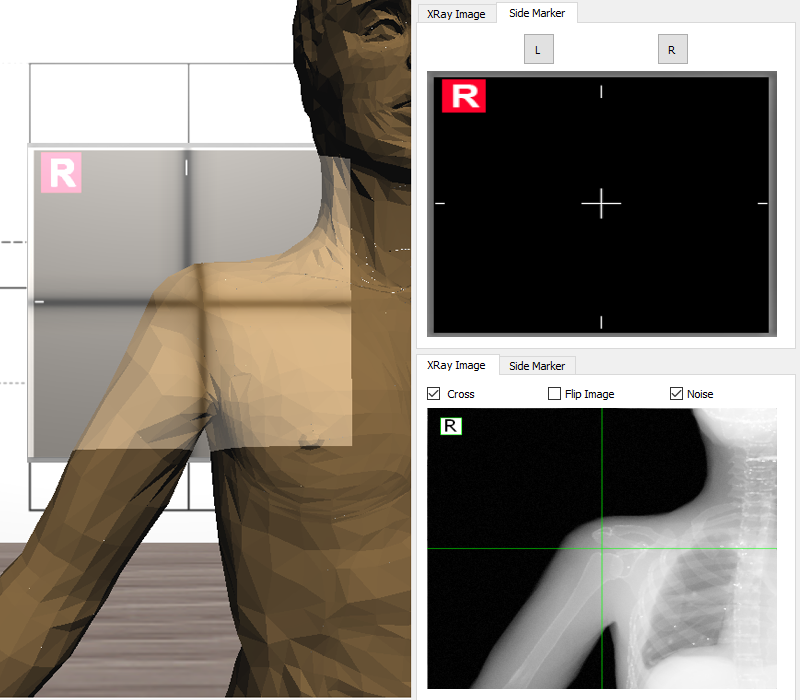
\includegraphics[width=\linewidth]{IMG/Rside.png}}
        \caption{Marcador de referencia derecho.}
    \end{subfigure}
    \null\hfill
     \begin{subfigure}[b]{0.45\linewidth}
        \centering
        {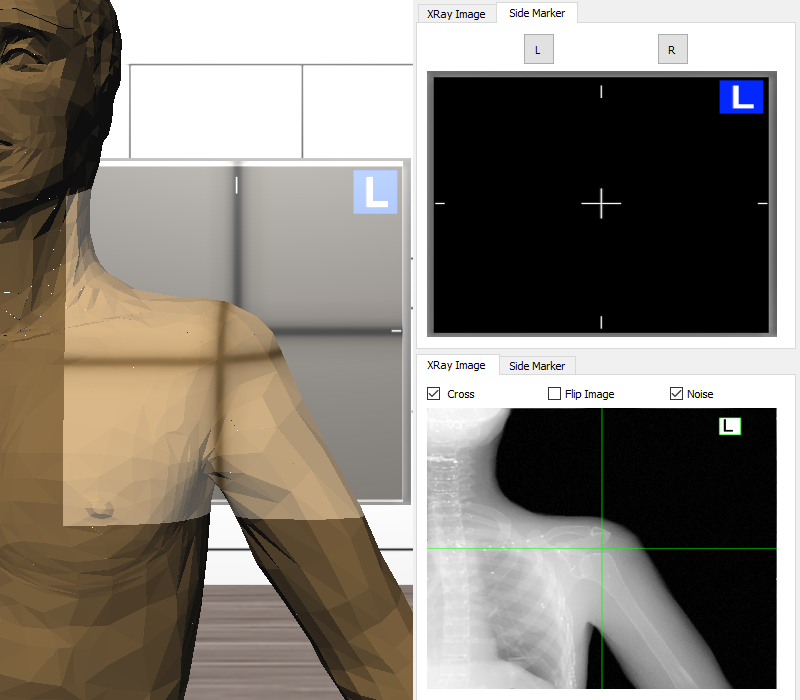
\includegraphics[width=\linewidth]{IMG/Lside.png}}
        \caption{Marcador de referencia izquierdo.}
    \end{subfigure}
    \caption{\label{fig:side} El usuario puede seleccionar y posicionar un marcador de referencia, que se trasladará a la escena 3D.}
   \end{figure}




\subsection{Manipulación digital de imágenes}
\label{xray:ajustes}

%En la sección \ref{xray:setupxray}, el usuario puede configurar y familiarizarse con el concepto de \ac{kVp} con el objetivo de mejorar la calidad de la radiografía resultante. 
En la actualidad, los detectores de los hospitales modernos son digitales y permiten capturar y almacenar la imagen radiológica de forma digital. Esta imagen digital se podrán mostrar en un ordenador instantáneamente. Quizás en el futuro, se podrán utilizar diagnósticos asistidos por computador, pero en la actualidad es necesario la intervención humana para interpretar las imágenes resultantes. La ventaja de la imagen digital es ofrecer la posibilidad de manipular la imagen médica. Esto permite, por ejemplo, a los usuarios tratar la imagen capturada con el objetivo de reducir los errores de sobre-exposición o sub-exposición producido por una mala configuración del emisor. Incluso, se puede conseguir más información de la imagen a través de aplicaciones de edición de imágenes que permiten observar detalles mínimos que no pueden verse a simple vista.  

Los usuarios pueden manipular y mejorar la imagen obtenida con algunas funcionalidades implementadas en el simulador. Se pueden cambiar el brillo y el contraste para enfatizar o remarcar las diferencias entre tejidos. Por otro lado, se han implementado un filtro gamma y un filtro logarítmico con el objetivo de mejorar la imagen capturada. Es posible también mostrar la imagen negativa o voltearla horizontalmente. El usuario puede modificar estos parámetros con el ratón y los botones integrados en la interfaz. En la figura \ref{fig:imgmani} muestra un ejemplo de manipulación de la misma imagen capturada. Por último, el usuario podrá elegir almacenar las imágenes manipuladas.% en \new{un} \del{el} disco duro.


% \begin{figure}[ht]
% \centering
% \includegraphics[width=0.5\linewidth]{IMG/imgmanipulation.png}
% \caption{\label{fig:imgmani} A: Imagen de referencia. B: Imagen en negativo. C: Imagen utilizando filtro Gamma. D: Imagen con filtro logarítmico. }
% \end{figure}

\begin{figure}[ht]
\begin{subfigure}[b]{0.3\linewidth}
        \centering
        {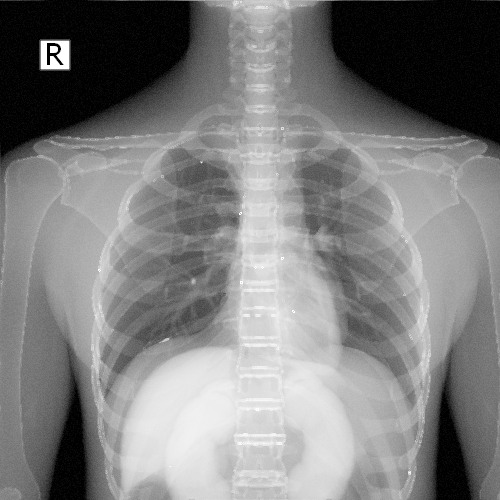
\includegraphics[width=\linewidth]{IMG/XRayMaleNormal2.png}}
        \caption{Imagen de referencia de  \emph{ZygoteBody}$^{TM}$. \label{xraynormal}}
    \end{subfigure}
    \null\hfill
    \begin{subfigure}[b]{0.3\linewidth}
        \centering
        {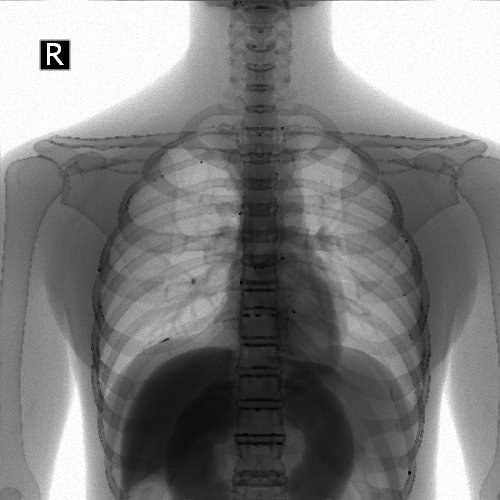
\includegraphics[width=\linewidth]{IMG/XrayMaleNegative2.png}}
        \caption{Imagen en negativo de la imagen \ref{xraynormal}.}
    \end{subfigure}
    \null\hfill
     \begin{subfigure}[b]{0.3\linewidth}
        \centering
        {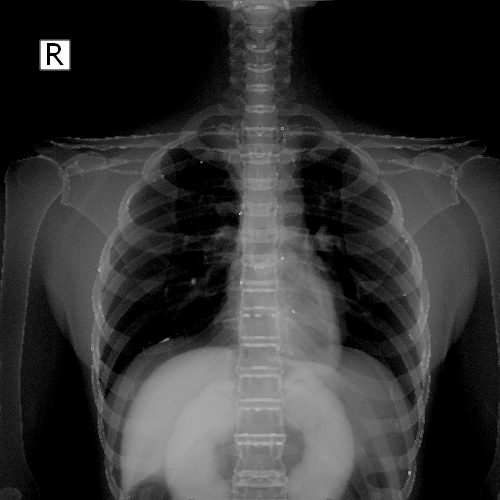
\includegraphics[width=\linewidth]{IMG/XRayMaleFilter2.png}}
        \caption{Imagen con un brillo bajo y un alto contraste.}
    \end{subfigure}
    \caption{\label{fig:imgmani}  Ejemplos de la misma proyección después de haber sido manipulado digitalmente.}
   \end{figure}



\subsection{Simulador como herramienta de clase}
\label{xray:sim}

%\subsection{Variedad de casos}
%\label{xray:variedad}
Se han desarrollado funcionalidades adicionales que, aunque no están directamente relacionadas con el procedimiento, permiten utilizar la herramienta como material de apoyo en las aulas. El profesor no solo podrá replicar las proyecciones mostradas en los archivos de imágenes y libros, sino que el simulador permite generar nuevas situaciones en comparación con los ejemplos estáticos.  %Pero, adicionalmente, podrá generar variaciones en el paciente virtual, modificando las propiedades de la anatomía o 
Los usuarios pueden ocultar ciertos tejidos en la ventana donde se muestra la escena 3D. De esta manera, el usuario podrá entender donde se sitúan o como se mueven los tejidos que se encuentran debajo de la piel. Incluso, es posible ocultar anatomía a la hora de simular la imagen radiográfica. De esta manera, se podría simular las imágenes resultantes en ausencia de ciertos tejidos. 

Otra ventaja que el simulador proporciona es la posibilidad de modificar la anatomía interna a través de sus propiedades físicas. Los usuarios pueden modificar la escala de \emph{Hounsfield} o la densidad del material descrito por su composición química para conseguir mostrar el efecto de ciertas enfermedades y su imagen radiológica asociada. Por ejemplo, un usuario puede calcificar un hueso, representar un pulmón colapsado o ilustrar como se vería un objeto extraño dentro del estómago como se puede ver en la figura \ref{fig:disease}. El simulador permite al usuario rotar y mover al paciente virtual para visualizar estos casos desde distintos ángulos de vista frente a la imagen estática mostrada en los archivos educativos y repositorios.%Esto podrá permitir al usuario visualizar diferentes variaciones desde infinidad de puntos de vista.


% \begin{figure}[ht]
% \centering
% 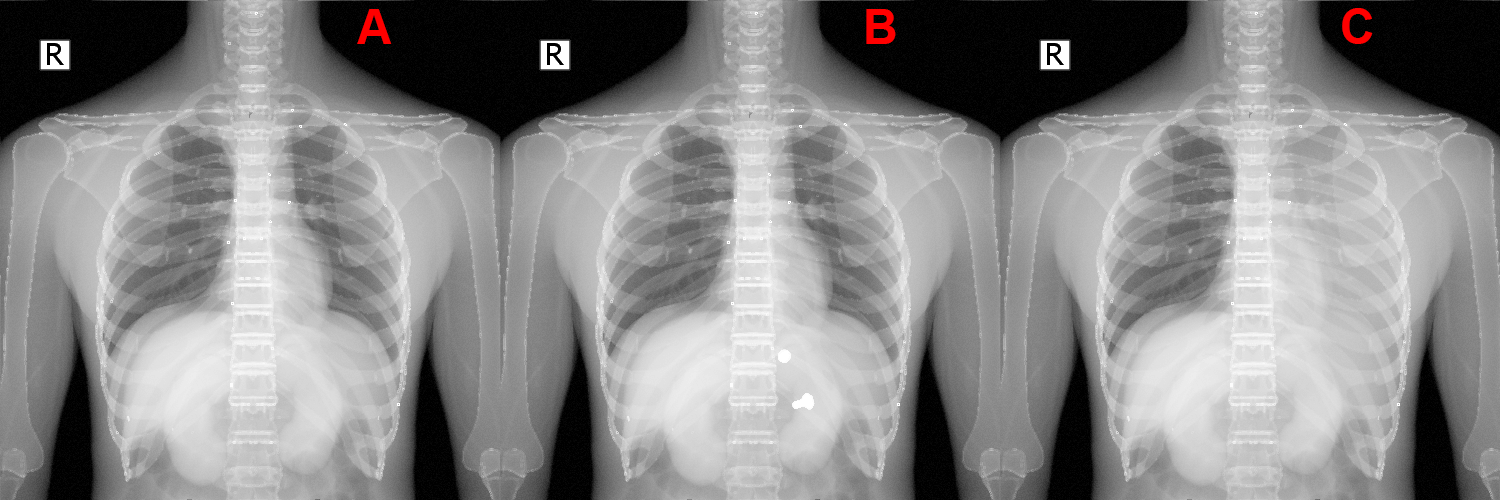
\includegraphics[width=0.5\linewidth]{IMG/disease.png}
% \caption{\label{fig:disease} Los usuarios pueden simular variedad de casos. A: Aspecto normal. B: Objetos extraños en el estómago. C: Pulmón izquierdo colapsado }
% \end{figure}

\begin{figure}[ht]
\begin{subfigure}[b]{0.3\linewidth}
        \centering
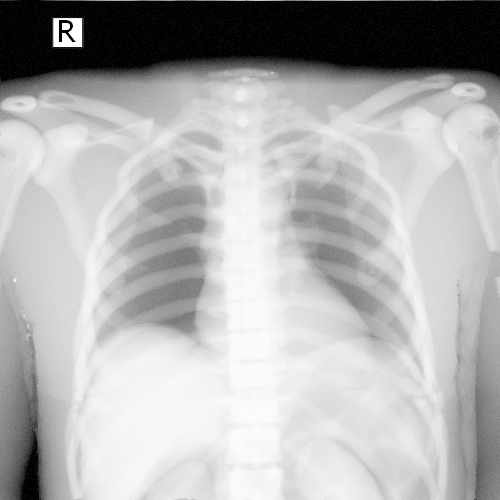
\includegraphics[width=\linewidth]{IMG/HVPForeign.png}
        \caption{Imagen  de \emph{Segmented Inner Organs} \cite{VoxelMan}.}
    \end{subfigure}
    \null\hfill
    \begin{subfigure}[b]{0.3\linewidth}
        \centering
        {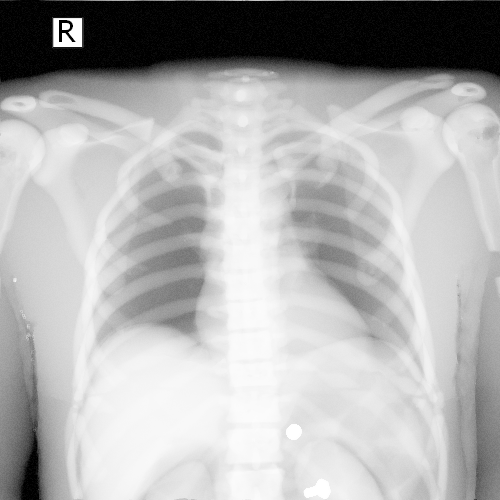
\includegraphics[width=\linewidth]{IMG/HVPNormal.png}}
        \caption{Objetos extraños en el estómago.}
    \end{subfigure}
    \null\hfill
     \begin{subfigure}[b]{0.3\linewidth}
        \centering
        {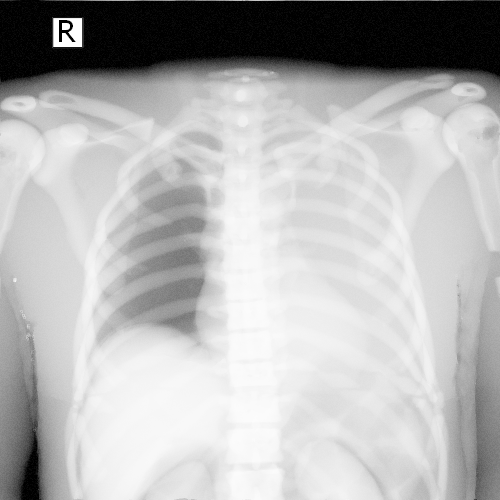
\includegraphics[width=\linewidth]{IMG/HVPLung.png}}
        \caption{Simulación de pulmón izquierdo colapsado.}
    \end{subfigure}
    \caption{\label{fig:disease} Un usuario puede ilustrar diferentes ejemplos con el mismo paciente virtual.}
   \end{figure}
   
   
Por otra parte, el profesor puede realizar una serie de proyecciones y guardar las imágenes obtenidas. Estas imágenes serán presentadas a los estudiantes para que averigüen cual es la proyección que se intenta conseguir y los parámetros que deberían ser usados para conseguir una imagen similar.

\subsection{Herramienta de aprendizaje autoguiado}

Con el objetivo de mejorar tanto sus habilidades cognitivas como las no cognitivas para realizar proyecciones radiológicas, los estudiantes pueden practicar la teoría en el simulador y mejorar su confianza en el procedimiento. En este contexto, los simuladores de \ac{RV} proporcionan el entorno seguro para enseñar o practicar procedimientos peligrosos para el paciente, pero es necesario una aplicación diseñada para guiar y mejorar el proceso de aprendizaje de los estudiantes. El simulador se ha diseñado para que se pueda utilizar de dos formas:
\begin{itemize}
    \item Orientado al estudiante: se ha diseñado un modo guiado que dirige al usuario durante el procedimiento y las funcionalidades del simulador. Este modo puede explicar cómo conseguir una buena proyección radiológica y ofrecer ayuda adicional al usuario si lo requiere. Antes de utilizar el simulador, el usuario puede revisar material multimedia que ayuda a familiarizarse con los elementos del simulador.
    
    \item Como método de evaluación, los estudiantes pueden realizar un ejercicio diseñado por sus profesores previamente. Los estudiantes deben realizar una lista de proyecciones concretas sin poder visualizar la imagen radiológica inmediatamente. El estudiante debe posicionar al paciente y configurar el emisor de rayos X al igual que haría en un entorno real. De esta forma, cuando estén seguros de su colocación, estos podrán tomar la radiografía. Los profesores pueden permitir repeticiones o no. El simulador guardará métricas de evaluación y las imágenes resultantes para que el profesor pueda evaluar al estudiante.
    
\end{itemize}





% \subsection{Caso de uso: Profesor}
% \label{xray:casodeuso}
% Los profesores imparten sus clases ayudados por presentaciones y siguen una lista de proyecciones radiológicas que quiere mostrar a los estudiantes. En el transcurso de la explicación de una proyección, el profesor puede cargar un modelo anatómico y enseñar interactivamente a realizar la proyección concreta.  Primero, el profesor explica la posición del paciente que debe tener para realizar la radiografía, moviendo las articulaciones que tenga el modelo disponible. A continuación explica cómo conseguir la configuración de la máquina de rayos X que permita conseguir la mejor imagen posible. El profesor puede centrarse en explicar cómo evitar los errores más comunes como una mala posición del centro de proyección, mala posición de marcadores de referencia, colimación pobre o una incorrecta configuración del emisor. Además, pueden realizar proyecciones incorrectas o posiciones incorrectas del paciente con la finalidad de que los estudiantes las identifiquen. Incluso, pueden simular enfermedades como la pancreatitis, piedras en el riñón o cuerpos extraños en la anatomía del paciente.


% \subsection{Caso de uso: Estudiante}

% Los estudiantes pueden usar esta herramienta como material adicional a sus libros y archivos de imágenes. Estos podrían revisar cada proyección explicada en el libro e intentar reproducirla en el simulador. Los estudiantes cargan un modelo anatómico y comienzan posicionando al paciente en su pose correcta. De pie, sentado, tumbado o mover cualquier articulación por separado si es necesario. Los estudiantes deberán configurar los parámetros del emisor de rayos X y centrar la proyección con forma de cruz proyectada por la luz del emisor, tal y como lo harían en un entorno real. Los estudiantes deben prestar atención a la colimación necesaria y poner el marcador de referencia en un sitio adecuado. La imagen médica resultante puede ser almacenada para ser utilizadas con otras intenciones.



% \subsection{Casos de uso: Ejercicios de clase}

% Los profesores pueden diseñar un ejercicio de clase en la herramienta. Se elaboran una lista con las proyecciones que se necesitan reforzar o evaluar y la herramienta les pedirá a los estudiantes realizarlas. Los estudiantes abren la aplicación que cargará el modelo anatómico automáticamente y se les solicitará que realicen una serie de proyecciones vistas en clase. Los estudiantes deberán realizar el procedimiento sin ver la imagen de rayos X intentando simular un entorno realista. Cuando el estudiante cree tener una buena proyección, puede obtener la imagen médica y el sistema le preguntará si está de acuerdo o quiere repetirla. Cuando el usuario considere que su proyección es correcta, la herramienta procederá con la siguiente y guardará un conjunto de métricas de evaluación junto con la imagen que serán evaluadas por el profesor. 


% Por otra parte, el profesor puede realizar una serie de proyecciones y guardar las imágenes obtenidas. Estas imágenes serán presentadas a los estudiantes para que averigüen cual es la proyección que se intenta conseguir y los parámetros que deberían ser usados para conseguir una imagen similar.

